\documentclass[12pt, spanish, a4paper]{article}

\usepackage[spanish]{babel}
\usepackage{anysize}
\usepackage[utf8]{inputenc}
\usepackage{amsmath}
\usepackage{tabularx}
\usepackage{graphicx}
\usepackage{epstopdf}
\usepackage{lipsum}
\usepackage[backend=bibtex,style=verbose-trad2]{biblatex}

% Configuration
\marginsize{2.5cm}{2.5cm}{2.25cm}{2.25cm}

\bibliography{Space_Cats} 

\title{Space Cats \\ Documento de diseño del videojuego}
\date{\today}
\author{Rafael Alcalde Azpiazu}

\begin{document}
	
	% Title
	\pagenumbering{gobble}
	\maketitle
	\newpage
	
	% Contents
	\tableofcontents
	\newpage
	
	% Document
	\pagenumbering{arabic}
	
	\section*{Historial de cambios}
	
	\subsection*{Revisión 1.0}
	
	\paragraph{26 Febrero 2017} He creado un borrador del documento.
	
	\subsection*{Versión 1.1}
	
	\paragraph{22 Abril 2017} He ido editado el documento, añadiendo la descripción y todas las ideas y consideración de cara a la creación de este videojuego. Espero que quede bien explicado.
	
	\subsection*{Versión 1.2}
	
	\paragraph{23 Abril 2017} He revisado las consideraciones y he empezado a describir el mundo y sus elementos (en concreto el apartado de Jugabilidad, Game Engine, Obstáculos y Power-ups).
	
	\newpage
	
	\section{Descripción}
	
	Space Cats (En adelante SC) es un videojuego Shoot'em Up espacial en un universo de fantasías con animales antropomorfos. Controlas una nave que está pilotada por un gato y tu misión es ir terminando una serie de niveles que van apareciendo conforme avances. \\
	
	Cada nivel constará de una serie de oleadas de naves enemigas, en donde la idea es que el jugador las destruya mediante diferentes armas que tiene su nave. Los enemigos darán puntos cada vez que sean destruidos. Una vez hecho, podrán arrojar algún power-up que hará cambiar el armamento de la nave, darle más vida o darle un multiplicador de puntos. \\
	
	En algunos niveles especiales, al final de estos podrá aparecer un enemigo más grande y con más vida, al que se le llamará Jefe del nivel, el cual arrojar más puntuación y mejoras para la nave una vez se destruya.
	
	\subsection{Consideraciones}
	
	Se que es un proyecto pequeño, pero me gustaría hacerlo bien desde el principio, con buenas prácticas y bien documentado. Se que va a ser un trabajo bastante grande para lo que el juego requiere, pero por lo menos aprendo a llevar un cierto orden y una metodología. \\
	
	Me gustaría que el juego estuviera destinado al público en general, sin ningún target en mente. Es por eso que el estilo debería ser lo más minimalista y atractivo posible. \\
	
	He pensado que el producto software va a estar a disposición de quien haga falta (tanto documentación como código) en un repositorio de GitHub. En principio estará mantenido como un proyecto de software libre. Es la mejor forma de trabajar, a pesar de que de momento solo lo esté haciendo yo. Cabe destacar que GitHub también me puede servir de Back-up. \\
	
	Por último, que no estoy muy seguro, me gustaría que el juego sea multiplataforma. En un primer momento para PC (estaba pensando en usar el motor gráfico de Löve, ya que Lua es el lenguaje que mejor conozco).
	
	\newpage
	
	\section{Mundo}
	
	En este apartado hablaré sobre el mundo y elementos de SC, explicando y dejando los conceptos centrales del juego, así como un resumen de las mecánicas que se implementarán sobre el.
	
	\subsection{Descripción}
	
	Como ya comenté, el videojuego tendrá temática de espacio, con naves, asteroides y demás elementos de la ciencia ficción.
	
	\subsection{Jugabilidad}

	El juego será plenamente de un jugador, habiendo la posibilidad de hacerlo multijugador, pero no es lo más importante. El jugador tendrá el control de una nave espacial, la cual podrá manejar en el eje horizontal y vertical. El jugador tiene un número de vidas que pueden disminuir o aumentar según la nave, una cantidad de puntos que subirá según destruya elementos del juego, y el arma activada en ese momento. Se podría dar el caso de que tuviera un escudo u otra bonificación en función de lo que recoja. \\
	
	Por el otro lado de la pantalla saldrán una serie u oleadas de enemigos, para los cuales el jugador tendrá a su disposición en todo momento un arma equipada con la que destruirlos. Esta pueden cambiar obteniendo objetos que expulsan los enemigos al destruirse [véase la sección Power-ups]. La idea es que en cada nivel del juego, los enemigos vayan variando. \\
	
	También se puede dar el caso de que salgan diferentes obstáculos, los cuales el jugador tendrá la posibilidad de poder esquivarlos o destruirlos. Al destruirlos, podrán arrojar objetos defensivos o curativos que podrá recolectar el usuario. En caso de esquivarlos, se le puede dar una serie de puntos al jugador en caso de no haber colisionado con ese objeto. \\
	
	Al final de los niveles, se podría dar el caso de que apareciera un Jefe del nivel, el cual sería un enemigo con una gran cantidad de vida y defensa. El objetivo del jugador en este caso sería destruirlo, momento en el cual se podría dar una gran bonificación, algún potenciador para el próximo nivel o incluso un premio.
	
	\subsection{Game Engine}
	
	\begin{figure}[!htb]
		\centering
		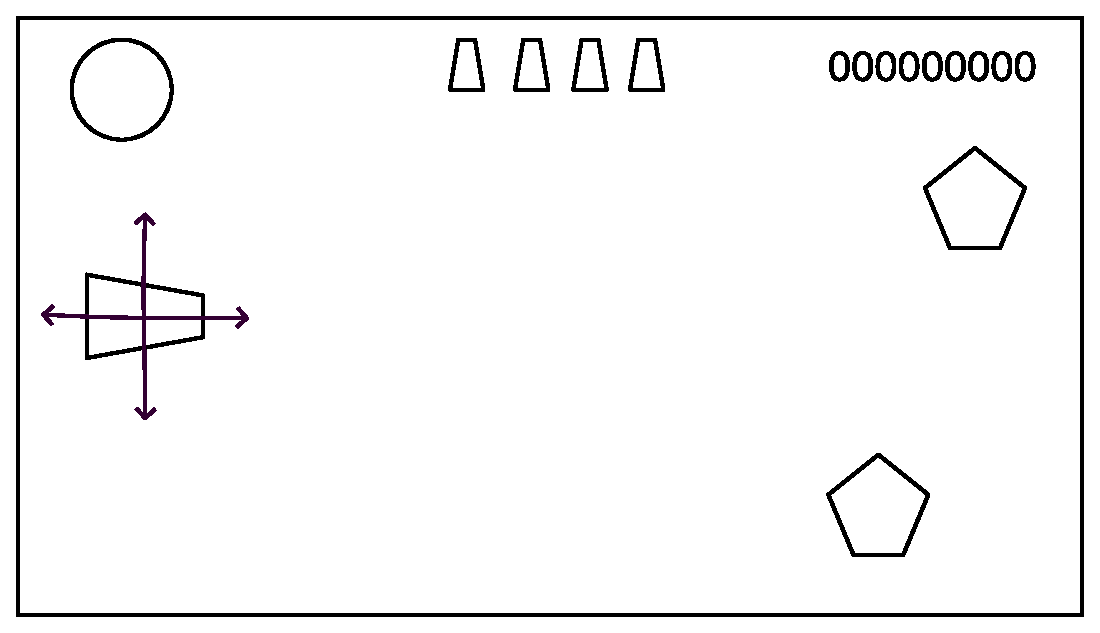
\includegraphics[scale=.5]{prototype.eps}
		\caption{Prototipo de la pantalla de juego}
		\label{fig:prototipo}
	\end{figure}
		
	Tal y como se ve en la figura \ref{fig:prototipo}, SC es un juego en dos dimensiones. He pensado que la mejor idea para su posterior implementación sea usar un motor gráfico ideal para mundos 2D. Lo ideal es que pudiera ser multiplataforma, ejecutándose en un primer momento en los diferentes sistemas operativos de escritorio y luego centrarse en llegar al resto de plataformas en el caso de que el proyecto sea viable. \\
	
	Es por eso que se ha pensado en utilizar Löve como motor, el cual reúne muchas de las características anteriormente mencionadas. El motor trabaja sobre el lenguaje de programación Lua (en concreto Lua 5.1), por lo que no va a ser mucho obstáculo al tener algo de experiencia en ese lenguaje. \\
	
	Los diseños de objetos en pantalla y escenarios serán imágenes planas con posibilidad de animación (tiles y sprites, que el caso de que se utilice el motor gráfico, se puede resolver mediante bibliotecas especializadas). En otra parte, la cámara será estática, siempre mostrando el juego desde una perspectiva lateral. \\
	
	El sistema de colisiones en este juego es realmente sencillo. El juego debe verificar si los disparos provenientes del jugador han colisionado con algún elemento (enemigo o obstáculo) en pantalla. También debe verificar si los disparos de los enemigos han colisionado contra la nave del jugador. Por último, deberá de comprobar si algún obstáculo ha colisionado con el jugador. \\
	
	Todo esto se puede resolver mediante colisiones de cajas para los elementos grandes y colisiones de punto-caja para tema de balas con un objeto grande. Si se utiliza el motor de juego propuesto, existen bibliotecas especializadas en este ámbito que se pueden usar para el ello.
	
	\subsection{Interfaz}
	
	\lipsum[13]
	
	\subsection{Escenarios}
	
	\lipsum[14]
	
	\subsection{Obstáculos}
	
	Los obstáculos son elementos grandes que salen en pantalla para entorpecer al jugador. Dependiendo del escenario, pueden ser de distintos tipos:
	
	\begin{itemize}
		\item Asteroide: Son rocas grandes que se mueven a gran velocidad y que tienen bastante defensa. Al destruirlas pueden fragmentarse y dividirse en trozos más pequeños.
		\item Cometa: Masas de hielo y roca que se mueven a gran velocidad. Tienen una cola de hielo por detrás de ellos. Podría darse el caso de que esta cola congele al jugador y quede unos segundos sin poder moverse.
		\item Satélite: Los satélites son máquinas que derivan por el espacio recolectando información. Algunas son replicantes, pudiéndose dividir en más. Otros están ya estropeados y no funcionan. Se podría dar el caso de que un satélite que no funcione electrocute al jugador y le cambie los controles durante unos segundos.
		\item Basura: Son elementos que van a la deriva en el espacio. No sirve para nada, solo hacen daño al jugador si colisionan contra ellos.
	\end{itemize}
	
	\section{Power-ups}
	
	Los power-ups o poteciadores son elementos recolectables que permiten al jugador cambiar de arma, añadir un escudo o conseguir un bonus de puntuación.
	
	\subsection{Defensivos}
	
	\begin{itemize}
		\item Escudo: Aumenta la defensa del jugador, reduciendo el daño recibido por el enemigo. Si el escudo está al máximo, no se aplica.
		\item Vida: Restaura la salud del jugador en caso de que haya perdido alguna vida. En caso de que no se haya perdido nada, no se aplica.
	\end{itemize}
	
	\subsection{Ofensivos}
	
	\begin{itemize}
		\item Multiplicador: Aumenta el daño recibido.
		\item Blaster: Armamento básico que consiste en balas de plasma ionizado que puede llegarse a disparar en intervalos regulares.
		\item Blaster mejorado: Consiste en balas de plasma ionizado muy pequeñas pero más calientes que pueden dispararse muy rápido.
		\item Electroblaster: Balas de plasma electricamente cargadas que pueden lanzar una descarga a los enemigos.
	\end{itemize}
	
	\subsection{Neutros}
	
	\begin{itemize}
		\item Multiplicador: Multiplica los puntos obtenidos durante un breve periodo
	\end{itemize}
	
	\section{Naves}
	
	\lipsum[18]
	
	\subsection{Naves del jugador}
	
	\lipsum[19]
	
	\subsection{Naves enemigas}
	
	\lipsum[20]
	
	\section{Arte}
	
	En este apartado hablaré sobre todo lo que tenga que ver con el diseño visual y sonoro del juego. Intentaré incluir las referencias a los archivos que se usarán, tanto creados por mi como todos aquellos que recoja de Internet.
	
	\subsection{Descripción}
	
	\lipsum[22]
	
	\subsection{Música}
	
	\lipsum[23]
	
	\subsection{Efectos de sonido}
	
	\lipsum[24]
	
	\subsection{Elementos}
	
	\lipsum[25]
	
	\subsection{Fondos de los escenarios}
	
	\lipsum[26]
	
	\subsection{Objetos}
	
	\lipsum[27]
	
	\section{Anexos}
	
\end{document}
